\chapter{Fast-ion Diagnostic Weight Functions}\label{chap:weights}

From a diagnostics standpoint, fast-ion physics is particularly difficult.
Unlike bulk-ion diagnostics that measure Maxwellian distributed velocities, fast-ion diagnostics  measure a velocity distribution that can be highly anisotropic due to neutral beam and RF heating.
The lack of a simple parametrization of the fast-ion velocity distribution makes it difficult to draw correlations between experimental data and the relevant fast-ion physics.
In an effort to aid the modeling, interpretation, and experimental design of fast-ion diagnostics, the following \textit{ansatz} was proposed\cite{heidbrink2007}
\begin{equation}\label{eq:vs_WF}
    S_{tot} = \iint W(E,p)F(E,p)\,dEdp
\end{equation}
where $S_{tot}$ is the total diagnostic signal, $F(E,p)$ is the fast-ion energy-pitch distribution function, and $W(E,p)$ is a diagnostic weighting function, colloquially known as the velocity-space weight function. The weight function indicates the phase-space sensitivity of the diagnostic, allowing for easier interpretation of the diagnostic data. As an aside, it is also common to formulate the weight functions in terms of the velocities parallel and perpendicular to the magnetic field, hence the name velocity-space weight functions. The transformation between the two coordinates is detailed in Appendix \ref{app:ep2vs}.

In the following sections, we will discuss how velocity-space weight functions are used and their limitations. We then show how to derive generalized diagnostic weight functions from the full forward models. With this firm theoretical footing, we also show how the generalized weight functions can be used to derive weight functions in guiding-center orbit space.

\section{Velocity-space Weight Functions}
Since their introduction, there has been a focused effort in calculating velocity-space weight functions for more fast-ion diagnostics\cite{salewski2011,salewski2014,jacobsen2015,salewski2015,salewski2016}. Figure \ref{fig:vs_weights} shows velocity-space weight functions, calculated by FIDASIM, for the neutron, NPA, and FIDA diagnostics. The velocity-space weight functions are used primarily to interpret diagnostic signals. While forward modeling can tell you \textit{what} the expected diagnostic signal should be, it provides little insight into the \textit{why}. Velocity-space weight functions provide a way to inspect diagnostic signals at a deeper level. 
\begin{figure}[ht]
    \centering
    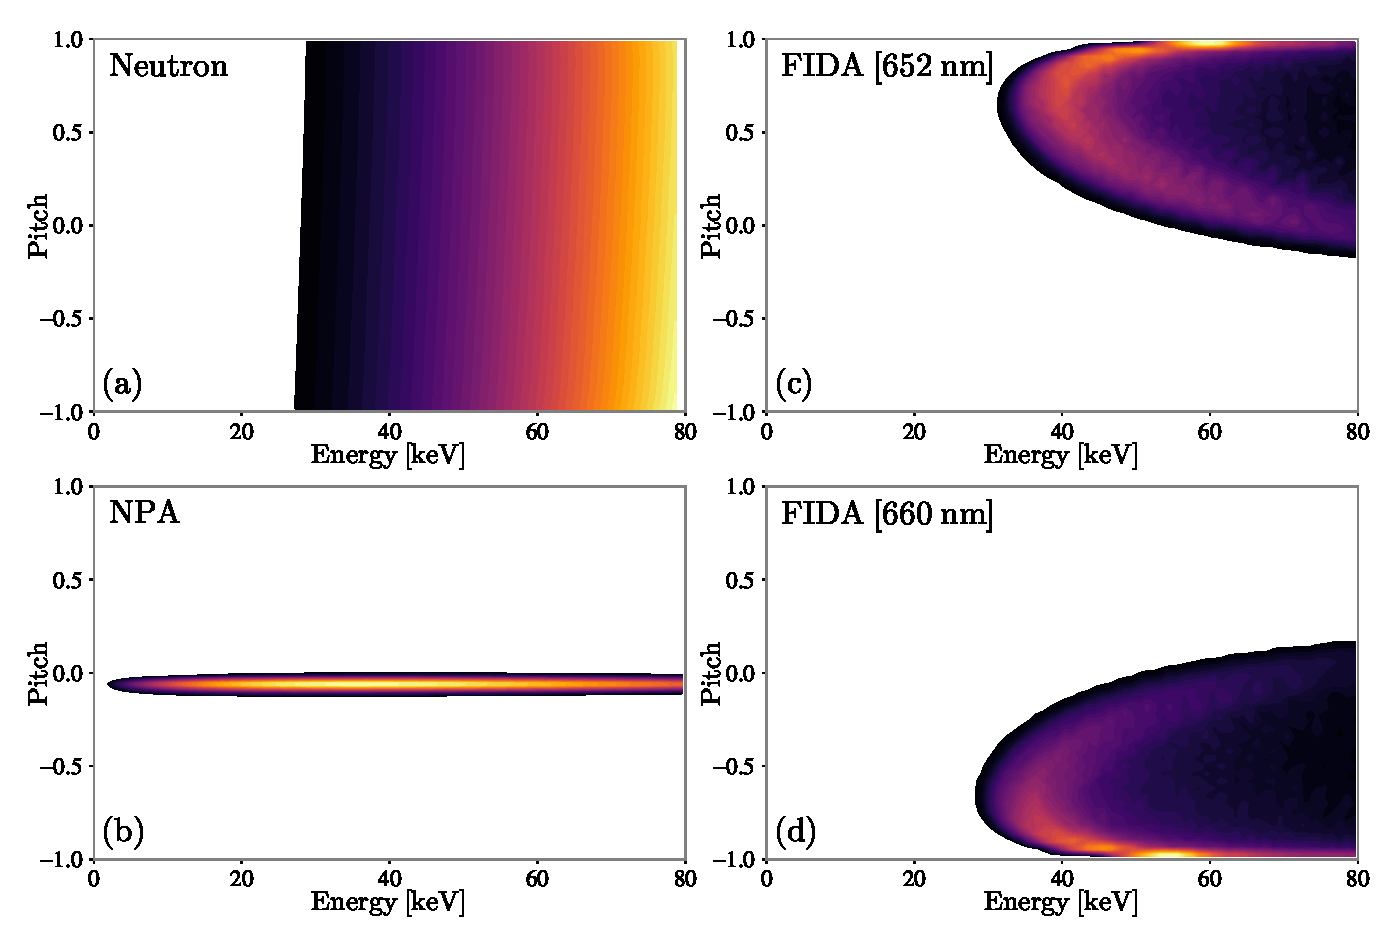
\includegraphics[width=13cm]{figures/velocity_space_weights.eps}
    \caption{Representative velocity-space weight functions for the DIII-D plasma and diagnostics. (a) The neutron scintillator is a global measurement of the neutron production rate. Its weight function for beam-plasma neutron production is spatially averaged and shows a strong energy dependence. The slight anisotropy in pitch is due to fast ions traveling with (positive pitch) and against (negative pitch) the plasma rotation. (b) The Neutral Particle Analyzer (NPA) diagnostic detects neutralized fast ions that escape the plasma. The collimation of the detector only permits a small range of pitch values to hit the detector and, because the detector is operated in current mode, the weight function is sensitive to many different energies. (c-d) The Fast-ion Deuterium-$\alpha$ (FIDA) diagnostic measures spectra produced by neutralized fast ions. The weight function 
depends upon wavelength. These FIDA weight functions are line-of-sight 
averaged at $\lambda = (652,660) \pm 0.2 \;\rm{nm}$ for a single oblique (Fig. \ref{fig:geometry}) viewing chord.}
    \label{fig:vs_weights}
\end{figure}

For instance, in an experiment at DIII-D, a modulated low power neutral beam was used to create an oscillating fast-ion population. The shot (\#157725) had minimal magneto-hydrodynamic (MHD) instabilities and was intended to be a baseline for later discharges. A radial array of FIDA chords---the oblique system in Fig. \ref{fig:geometry}---was used to monitor the oscillating fast-ion population. Figure \ref{fig:fida_waveform} shows FIDA waveforms conditionally averaged over four 54ms oscillation periods for the different radial positions. Figures \ref{fig:fida_waveform_low} and \ref{fig:fida_waveform_high} show the waveforms for data integrated over small and large Doppler shifts respectively. 
\begin{figure}[ht]
    \centering
    \subfigure[][]{%
        \label{fig:fida_waveform_low}
        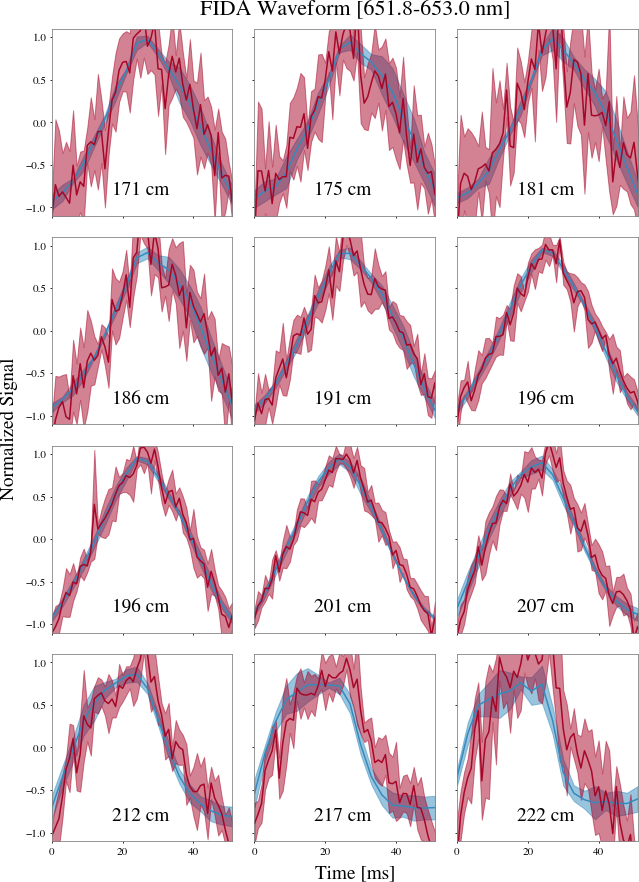
\includegraphics[width=7cm]{figures/FIDA_waveform_21_40_kev.png}}
    \hspace{2pt}
    \subfigure[][]{
        \label{fig:fida_waveform_high}
        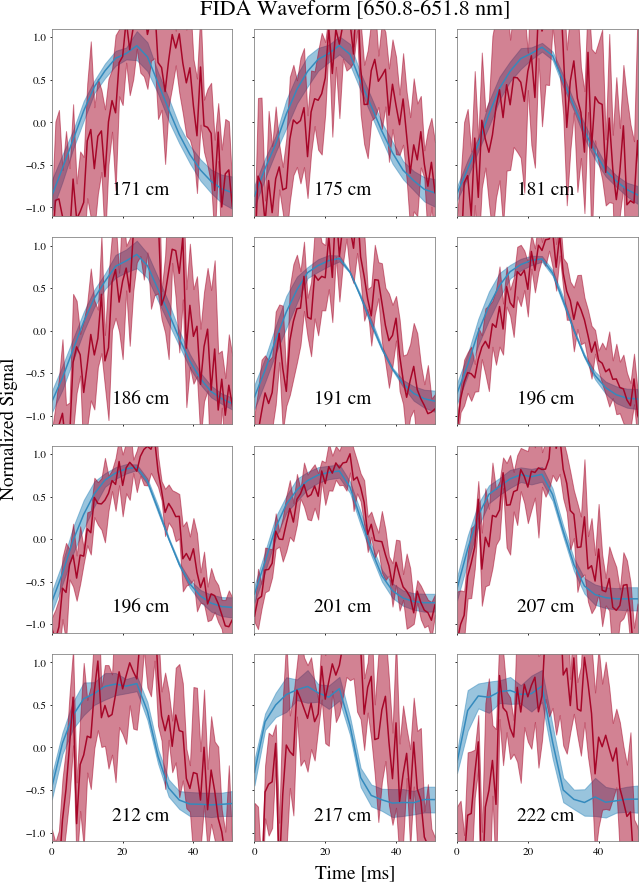
\includegraphics[width=7cm]{figures/FIDA_waveform_40_61_kev.png}}
    \caption{FIDA waveforms for DIII-D shot \#157725 for two different integration ranges:
        \subref{fig:fida_waveform_low} Small Doppler shift/alpha waveform: $\Delta \lambda = 651.8-653.0\;nm$;
        \subref{fig:fida_waveform_high} Large Doppler shift/beta waveform: $\Delta \lambda = 650.8-651.8\;nm$.
        FIDA data and error-bars averaged over four oscillation periods are shown in red, the corresponding weight function calculated theoretical signals are shown in blue. Errors in the theoretical signals derive from varying plasma profiles over the different periods. The neutral beam is on during the first half of the period and off during the second half.}
    \label{fig:fida_waveform}
\end{figure}

Despite looking at the same radial location, the waveforms for the small and large Doppler shifts, which will henceforth be called the alpha and beta waveforms respectively, are different. In the core region ($\sim181$ cm), the alpha waveform slowly increases in the first half of the period, when the beam is on, and slowly decays in the second half, when the beam is off. The beta waveform shows the opposite trend: growing quickly when the beam is on and decaying quickly when it is turned off. Forward modeling alone is unable to explain the different trends. Velocity-space weight functions, however, allows us to determine where in velocity-space the signal is originating. Figure \ref{fig:fida_waveform_WF} compares the waveforms at $R=181$ cm and shows the corresponding time evolution of the products of the velocity-space weight functions and the local theoretical distribution, $W(E,p)\times F(E,p)$.
\begin{figure}[h!]
    \centering
    \includegraphics[width=15cm]{figures/FIDA_waveform_compare.eps}
    \caption{Weight function analysis: Top row: comparison of the FIDA waveforms for small/alpha (red line) and large/beta (blue line) Doppler shifts at $R=181$ cm. Colored dashed lines are the data. Middle row: time evolution of the product of the large Doppler shift velocity-space weight function and the local theoretical distribution function. Bottom row: time evolution of the product of the small Doppler shift velocity-space weight function and the distribution function. The color-maps increase linearly from light to dark. The distribution function is calculated using the TRANSP/NUBEAM\cite{NUBEAM} code.}
    \label{fig:fida_waveform_WF}
\end{figure}
The weight functions in Figure \ref{fig:fida_waveform_WF} are sensitive to different regions in phase-space. The alpha weight function is only sensitive to fast ions with energies greater than $\sim$40keV, while the beta weight function is sensitive to lower energies, $>$20keV. If we take the weight functions to have a similar pattern of sensitivity as Figure \ref{fig:vs_weights}c the reasons for the shape of the waveforms are apparent. For the beta waveform, the fast-ions are born into a higher sensitivity region and move into regions of zero sensitivity. Comparatively, for the alpha waveform the fast ions are born in a low sensitivity region and move into higher sensitivity regions as they slow down. This results in a quicker growth in the beta waveform and slower growth in the alpha waveform. When the beam is turned off in the middle of the period the alpha waveform decays slowly due to a large fraction of the fast-ions still in the weight function's sensitive region. For similar yet opposing reasons, the beta waveform decays more quickly when the beam is turned off.

In addition to enhancing our ability to analyze experimental data, velocity-space weight functions provide a method of inferring the local fast-ion distribution function\cite{salewski2013_tomography,salewski2014_tomography}. Equation \ref{eq:vs_WF} can be discretized, creating a system of linear equations. When multiple diagnostics view the same spatial location, the system of linear equations can be solved via various numerical methods\cite{jacobsen_stagner2016}. This application of weight functions will be discussed in depth in the next chapter.

Velocity-space weight functions have enhanced our ability to understand diagnostic signals and, through Velocity-space Tomography, the fast-ion distribution function itself. However, velocity-space weight functions are hindered, both in their accuracy and in their practicality due to the implicit assumption that diagnostic signals are spatially localized. The flaws in this assumption can be made plain by comparing the diagnostic signals calculated using FIDASIM and Equation \ref{eq:vs_WF}.
\begin{figure}[h!]
    \centering
    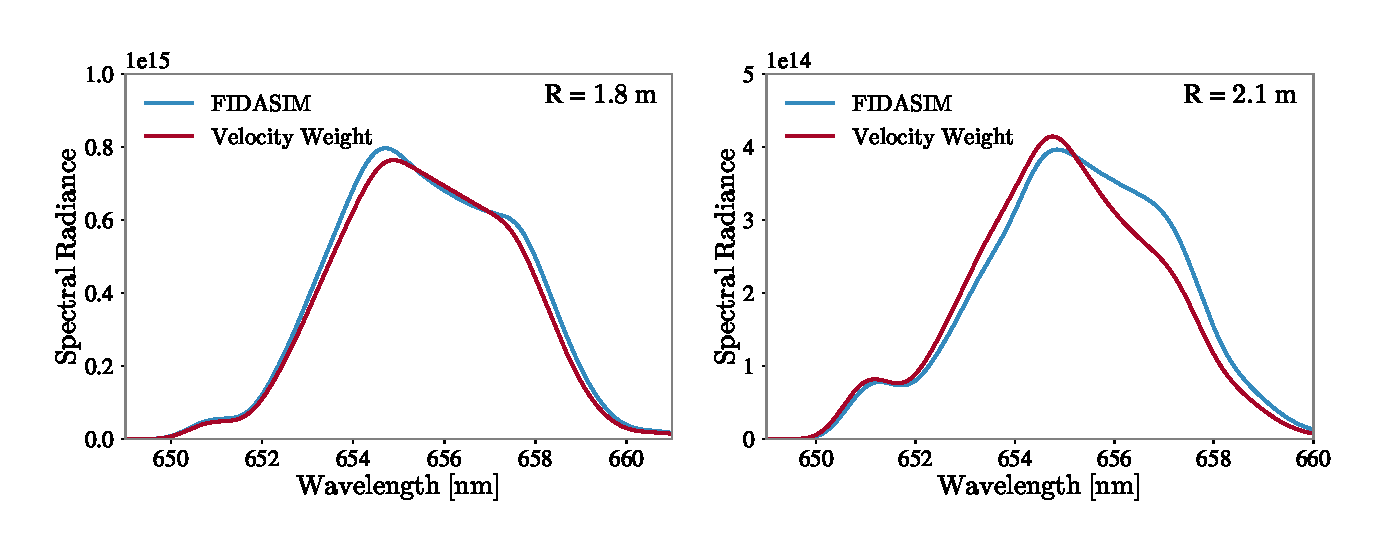
\includegraphics[width=15cm]{figures/fida_spectra.eps}
    \caption{FIDA spectra calculated using velocity-space weight functions 
(Equation~\ref{eq:vs_WF}) for the oblique viewing chords at
(a) $R = 1.8$ and (b) $R = 2.1$ m.  The spectra calculated by FIDASIM are also shown.
 Disagreement between FIDASIM and Equation \ref{eq:vs_WF} is because the latter uses a local fast-ion distribution to calculate the spectra. Differences between the local distribution and the full distribution used by FIDASIM cause the two methods to disagree to varying degrees.}
    \label{fig:fida_spectra}
\end{figure}
In regions where the fast-ion distribution has large spatial variations, velocity-space weight functions perform poorly.
Figure~\ref{fig:fida_spectra} shows spectra calculated using spatially-averaged velocity-space
weight functions.  Near the magnetic axis (Fig.~\ref{fig:fida_spectra}a), the calculated
spectrum agrees fairly well with FIDASIM, indicating that the velocity-space weight function method is fairly accurate. However,
off-axis (Fig.~\ref{fig:fida_spectra}b), the spectrum calculated with
velocity-space weight functions deviates significantly from FIDASIM.  Comparisons with simulations that use an uniform fast-ion distribution are not discrepant, showing that spatial variations are responsible for the deviation.
Generally, as in Figure \ref{fig:fida_spectra}, velocity-space weight functions agree with FIDASIM in the core, where spatial gradients are relatively smaller, than in the periphery, where variations in the fast-ion density and other quantities tend to be large.
This trend is also seen in Figure \ref{fig:fida_waveform}.

Another mark against velocity-space weight functions is that velocity-space tomography requires overlapping diagnostic views.
In practice, due to limited port access, radial arrays from one or two ports are more common than multiple views of the same spatial volume from different viewing locations. 
To resolve these crippling limitations, a generalization of Equation \ref{eq:vs_WF} to include spatial dependencies needs to be derived.

\section{Generalized Diagnostic Weight Functions} \label{sec:generalized_weight}
Velocity-space weight functions are typically derived using variations of probabilistic arguments\cite{salewski2011,salewski2014,jacobsen2015,salewski2015,salewski2015}. When considering a fixed location within the plasma, a probabilitic approach is often simpler. However, in order to properly account for the spatial dependencies of the diagnostics, a different tack is needed.

Consider a fast ion with phase-space coordinates $\mathbf{x} = [\mathbf{p},\mathbf{q}]$, where $\mathbf{p}$ and $\mathbf{q}$ are the generalized momentum and position, respectively.
As seen in Chapter \ref{chap:diagnostics}, the forward models for many fast-ion diagnostics can be expressed as a function, $S(\mathbf{x})$, which gives the expected signal produced by a fast ion with phase-space coordinates $\mathbf{x}$.
The total diagnostic signal is found by summing the contributions of all the individual fast ions,
\begin{equation}\label{eq:sum_S}
    S_{tot} = \sum_{k=1}^N S(\mathbf{x}_k),
\end{equation}
where $N$ is the total number of fast ions in the plasma.
This equation can be expressed in terms of the frequency in which $\mathbf{x}$ occurs
\begin{equation}\label{eq:sum_SP}
    S_{tot} = N \sum_{\mathbf{x}_k \in R_{X}} S(\mathbf{x}_k) P_X(\mathbf{x}_k),
\end{equation}
where $P_X(\mathbf{x}_k)$ is the frequency of $\mathbf{x}_k$ occurring.
In the continuum limit, the discrete sum in the above equation can be replaced by an integral and can be written in the form
\begin{equation}\label{eq:SF}
    S_{tot} = \int S(\mathbf{x})\,N \sum_{\mathbf{x}_k \in R_{X}} P_X(\mathbf{x}_k) \delta(\mathbf{x} - \mathbf{x}_k) d\mathbf{x} = \int S(\mathbf{x}) F(\mathbf{x}) d\mathbf{x},
\end{equation}
where $F(\mathbf{x})$ is the fast-ion distribution function.
By inspection, it is clear that Equation \ref{eq:SF} is the generalized version of equation \ref{eq:vs_WF}.

Upon comparing Equation \ref{eq:SF} with how FIDASIM simulates the diagnostics it is apparent that they are equivalent as FIDASIM evaluates Equation \ref{eq:SF} via Monte Carlo integration.
\begin{equation}
    S_{tot} \approx \frac{1}{N_t} \sum_i^{N_t} S(\mathbf{x}_i)\quad \rm{where}\; \mathbf{x}_i \sim F(\mathbf{x})
\end{equation}
where $N_t$ is the number of FIDASIM's ``trajectories'', which just correspond to samples, $\mathbf{x}_i$, from the distribution function, $F(\mathbf{x})$. In fact, FIDASIM's neutral density calculations can also put into the form of Equation \ref{eq:SF} where, instead of the fast-ion distribution, the distribution function is either the neutral beam distribution, for the beam density calculation, or the thermal ion distribution, for the direct charge exchange and halo densities.

From the generalized form, we can also derive the velocity-space weight functions.
Consider the phase-space coordinate system $\mathbf{x} = \{E,p,\gamma, R, Z, \phi\}$, where $E$ is the energy, $p$ is the pitch with respect to the plasma current ($p=v_{\parallel}/v$), $\gamma$ is the gyro-angle, $R$ is the major radius, $Z$ is the elevation, and $\phi$ is the toroidal angle, the velocity-space weight function in Equation \ref{eq:vs_WF} can be recovered by averaging over the phase-space variables $R$, $Z$, $\phi$, and $\gamma$.\footnote{To remind readers, averaging over a variable in a function involves integrating over the product of the function and the probability of the variable. For example, $g(x) = \int f(x,y)p(y)dy$ is averaging $f(x,y)$ over $y$.}
Since most velocity-space weight functions are gyro-averaged and spatially localized the following reduction of equation \ref{eq:SF} reproduces the velocity-space weight function:
\begin{equation}\label{eq:vs_reduction}
    W(E,p) = \frac{1}{2\pi} \iiiint S(E,p,\gamma,R,z,\phi)\delta(R-R_0)\delta(z-z_0)\delta(\phi - \phi_0)\,d\gamma\, dR\, dz\, d\phi.
\end{equation}
At this point, we come to a clear understanding of what a velocity-space weight function actually is. A velocity-space weight function is the average signal produced by a fast ion with a given energy and pitch. 

\section{Orbit Weight Functions}\label{sec:orbit_weight}
A reduction of the phase-space, as done in Equation \ref{eq:vs_reduction}, greatly simplifies analysis and facilitates tomographic reconstructions by reducing the number of unknown parameters.
However, since we are concerned about the motion of the fast ions, care must be taken to ensure that no critical information is lost when averaging over variables.
In other words, only variables that do not appear in the Lagrangian (i.e. ignorable or cyclic coordinates) can be averaged out without critical information loss.
By this standard, the phase-space reduction done in Equation \ref{eq:vs_reduction} is inadequate since only the gyro and toroidal angle averaging was permissible. 

In order to reduce the phase-space as much as possible without sacrificing model fidelity, it is advantageous to express the expected diagnostic signal, $S$, in canonical action-angle coordinates, $\mathbf{x} = (\mathbf{J},\mathbf{\Theta})$.
Action-angle coordinates are a set of canonical coordinates with the special property that the action variables, $\mathbf{J}$, are invariants of the motion and the angle coordinates, $\mathbf{\Theta}$, are cyclic/ignorable and can, therefore, be safely averaged over when reducing the phase-space. 
In these coordinates, information preserving phase-space reductions can then be succinctly expressed as
\begin{equation}\label{eq:action_angle_reduction}
    W(\mathbf{J}) = \left( \prod_i \frac{1}{\tau_i} \right) \int_0^{\tau_1}\ldots\int_0^{\tau_i} S(\mathbf{J},\mathbf{\Theta})\, d\mathbf{\Theta}
\end{equation}
where $\tau_i$ are the periods of the angle coordinates and $W(\mathbf{J})$ is the action-space weight functions which is interpreted to be the average signal produced by a fast ion with action coordinates $\mathbf{J}$, similar to the velocity-space weight functions. 

The total diagnostic signal can be calculated using these action-space weight functions. Consider the subset of fast ions in a plasma with action coordinates, $\mathbf{J}_k$.
The signal produced by these fast ions is given by
\begin{equation}\label{eq:orbit_tomography_discrete}
    S_k = \sum_i^{N_k} S(\mathbf{J}_k,\mathbf{\Theta}_i) = N_k \sum_i^{N_k} S(\mathbf{J}_k,\mathbf{\Theta}_i)/N_k
\end{equation}
where $N_k$ is the number of fast ions with action coordinates $\mathbf{J}_k$.
The sum on the right-hand side is the average signal produced by the subset of fast ions. This is identical to the interpretation of the action-space weight function.
The total diagnostic signal can then be expressed as a linear combination of weight functions,
\begin{equation}\label{eq:orbit_tomography}
    S_{tot} = \sum_k N_k W(\mathbf{J}_k) .
\end{equation}
In the context of guiding center motion, $\mathbf{J}_k$ acts as a label for an individual fast-ion orbit. Therefore, Equation \ref{eq:orbit_tomography} can be interpreted as a sum of the signal produced by each fast-ion orbit.
As in velocity-space tomography, when there are multiple measurements, Equation \ref{eq:orbit_tomography} can be put into matrix form, creating a system of linear equations that can be solved. This is discussed in Chapter \ref{chap:orbit_tomography}.

An action-angle parametrization of the guiding center motion of a fast ion in a tokamak has three action coordinates and three angle coordinates.
There are many possible choices for action-angle coordinates; the classical choice being the canonical constants of motion: energy, magnetic moment, and toroidal canonical angular momentum, $\mathbf{J} = (E,\mu,p_\phi)$.
However, due to an ambiguity in the sign of $v_\parallel$ in the definition of $p_\phi$, the classical choice of coordinates does not always \textit{uniquely} label distinct orbits, i.e. a single action coordinate $ \mathbf{J}_k$ in this space could correspond to two different orbit trajectories i.e. orbit degeneracy. This can be plainly seen by expressing the magnetic moment as a function of the energy and toroidal angular momentum. 
\begin{equation}\label{eq:mu}
\mu(R,Z) = \frac{E}{B(R,Z)} - \frac{B(R,Z)}{2m} \left ( \frac{p_\phi - q\Psi(R,Z)}{RB_\phi(R,Z)}\right)^2
\end{equation}
Isolines of this function are the orbit trajectories for a fixed $\mu$, $E$ and $p_\phi$.
\begin{figure}[h!]
    \centering
    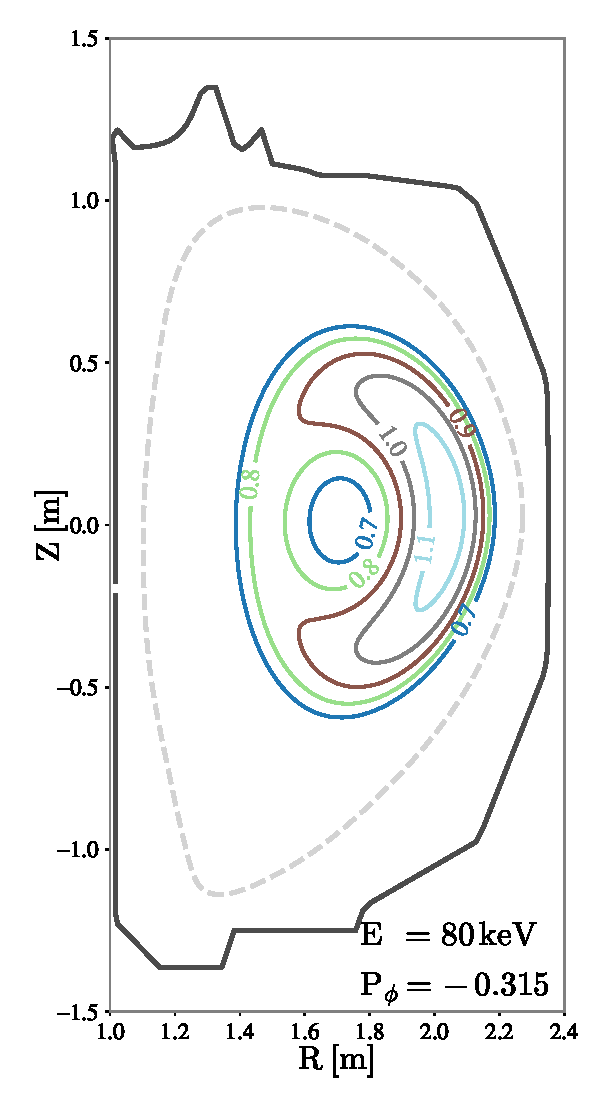
\includegraphics[width=7cm]{figures/hamiltonian_orbits.eps}
    \caption{Orbit trajectories generated by a scan of normalized magnetic moments, fixing energy (80 keV) and normalized canonical angular momentum (-0.315). Orbits are labeled by their normalized magnetic moments. Orbits with normalized magnetic moments of 0.7 and 0.8 are degenerate.}
    \label{fig:hamiltonian_orbits}
\end{figure}
Figure \ref{fig:hamiltonian_orbits} shows a scan over $\mu$ for a fixed $E$ and $p_\phi$. The scans show distinct orbits that have the same Hamiltonian coordinates.
The large distance between the orbits indicate that their fast-ion populations are independent and should be treated separately.
Orbit degeneracy also makes it impossible to use Equation \ref{eq:action_angle_reduction} to reduce the phase-space since the angle variables of the two orbits would have different periods.

To avoid this problem, we use a modified version of the coordinates first promoted by Rome\cite{rome1979} and others\cite{petrov2016}.
Here we define the action coordinates, hereby called orbit-space coordinates, to be
\begin{equation}\label{eq:orbit_action}
    \mathbf{J} = (E, p_m, R_m)
\end{equation}
where $E$ is the energy, $R_m$ is the maximal radius along the orbit, and $p_m$ is the pitch with respect to the plasma current at $R_m$.
The angle variables, which describe the position of the fast ion along the orbit, are
\begin{equation}\label{eq:orbit_angle}
    \mathbf{\Theta} = (t, \gamma, \phi_0)
\end{equation}
where $t$ is the time, $\gamma$ is the gyro-angle, and $\phi_0$ is the initial toroidal angle.
Applying Equation \ref{eq:action_angle_reduction} yields the definition of an orbit weight function,
\begin{equation}\label{eq:orbit_weight}
    W(E,p_m,R_{m}) = \frac{1}{4\pi^2 \tau_p}\int_0^{2\pi} \int_0^{2\pi} \int_0^{\tau_p} S(E,p_m,R_{m},t,\gamma,\phi_0)\,dt\, d\gamma d\phi_0
\end{equation}
where $\tau_p$ is the poloidal transit time.

This choice of orbit-space coordinates has several nice properties. The space has natural boundaries in all three coordinates ($E = [0,E_{max}]$, $R_m = [R_{axis},R_{wall}]$, and $p_m = [-1,1]$),
 which makes it easy to enumerate all possible orbit trajectories for a given magnetic equilibrium.
Additionally, as can be seen in the topological map of the orbit-space in Fig. \ref{fig:orbit_topology}, counter-passing orbits are easily identified by the sign of $p_m$.
\begin{figure}[ht]
    \centering
    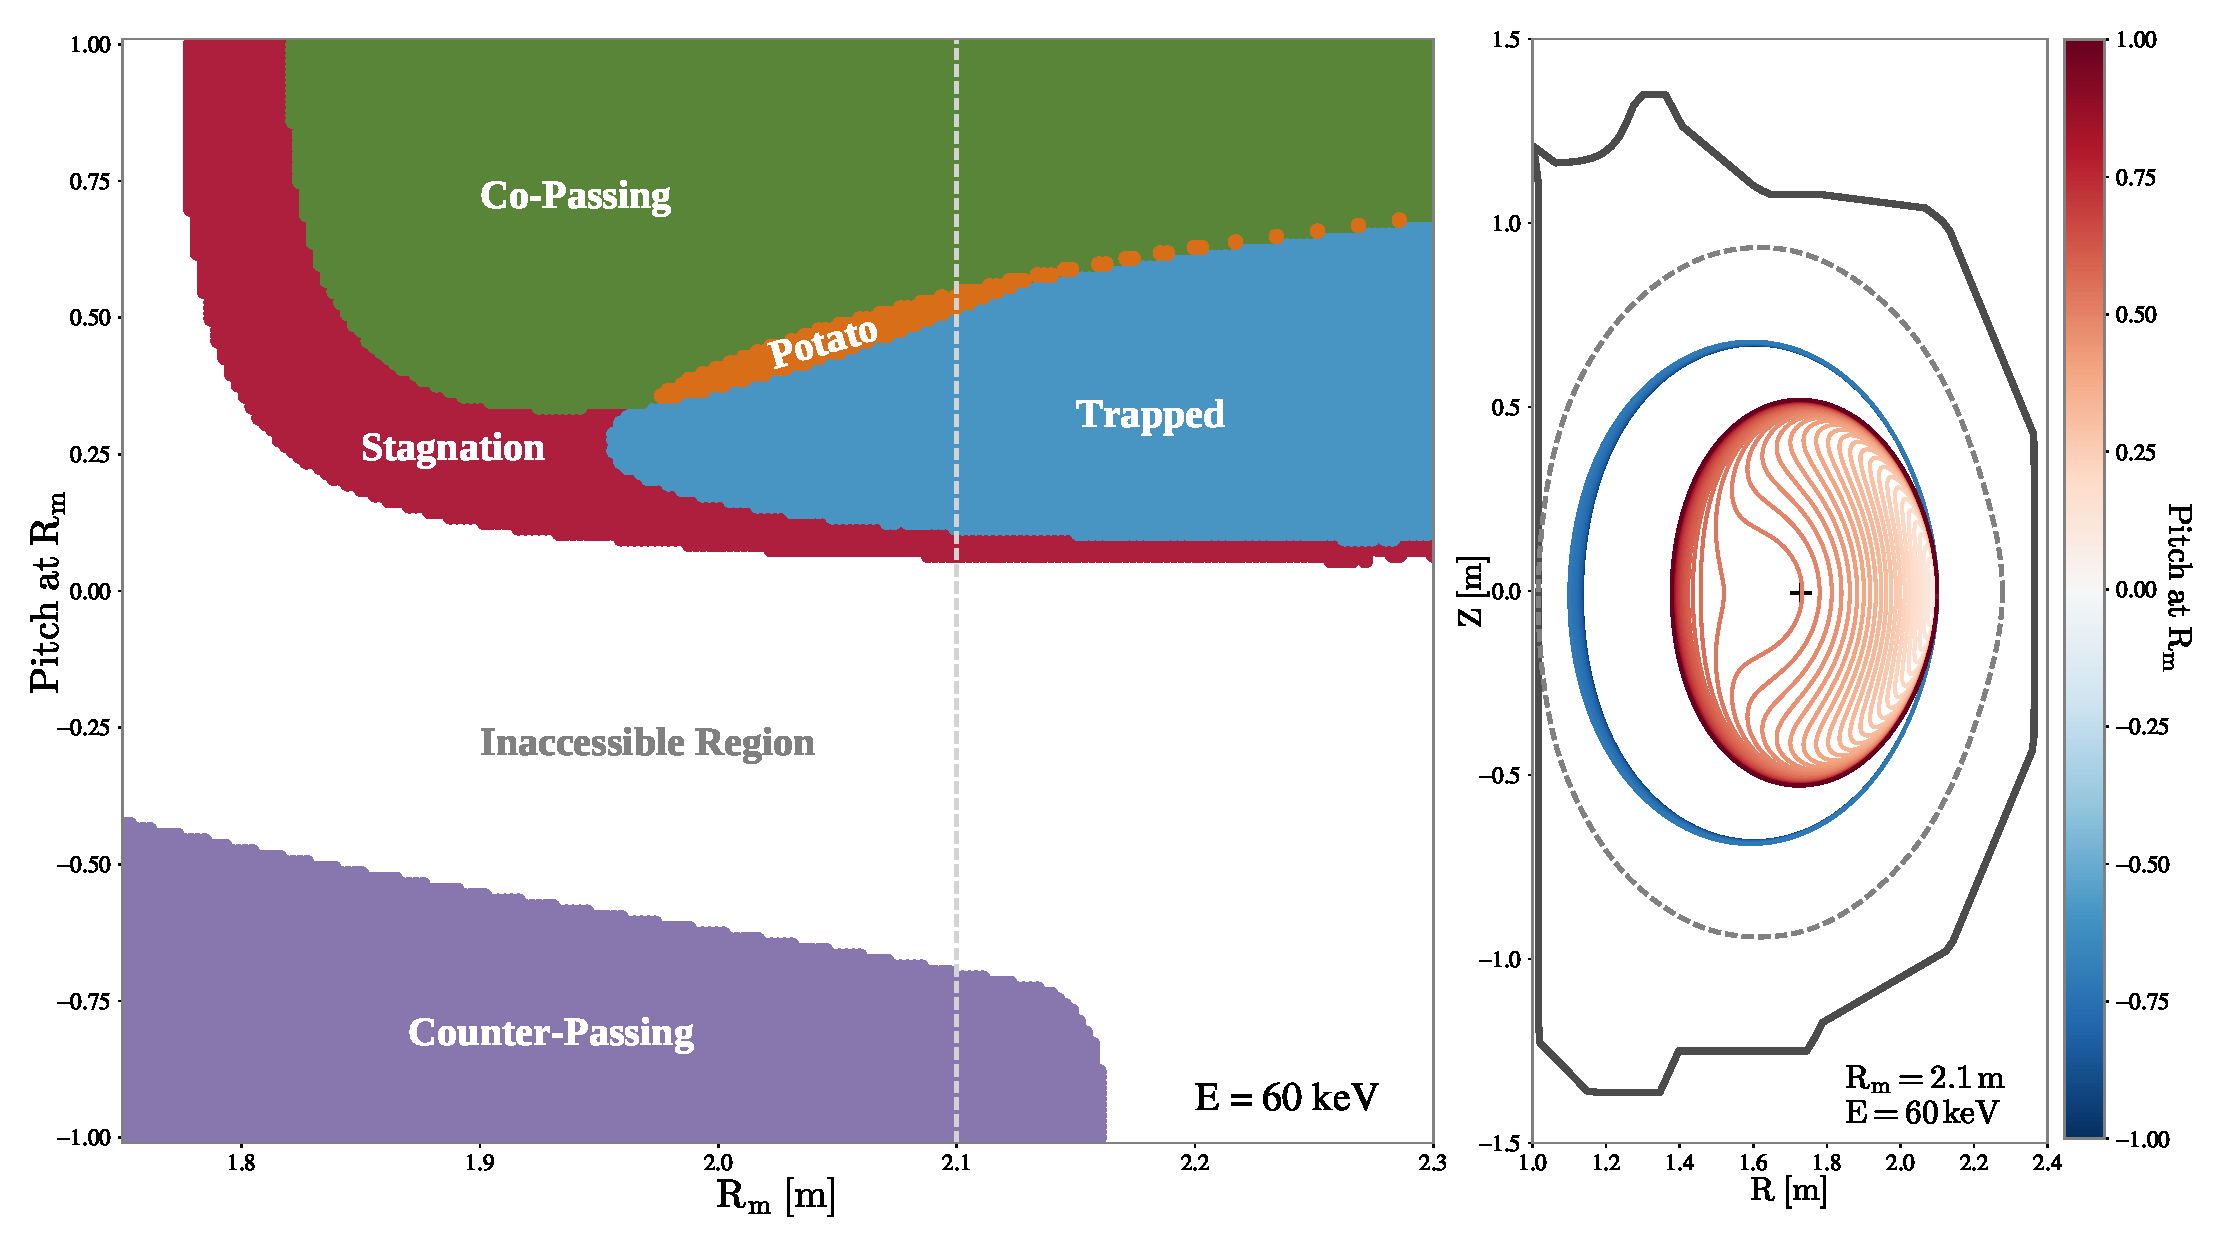
\includegraphics[width=15cm]{figures/orbit_topology3.eps}
    \caption{Left: Topological map of different orbit types \cite{WHITE} with fixed energy
for the DIII-D plasma described in Sec.~\ref{sec:apparatus}.
 \newline Right: Orbits corresponding to the dashed line in the topological map. The
plus indicates the magnetic axis and the dashed line is the last-closed flux surface. Counter-passing orbits have negative pitch along their orbit, while co-passing orbits have constant positive pitches. Stagnation orbits are co-passing orbits that do not enclose the magnetic axis. The pitches of fast ions on a trapped orbit change signs and potato orbits are trapped orbits that enclose the magnetic axis.}
    \label{fig:orbit_topology}
\end{figure}

\subsection{Numerical Calculation of Orbit Weight Functions}
As the name suggests, fast-ion orbits are needed to calculate orbit weight functions. The orbit trajectories are found by solving the guiding-center drift orbit ordinary differential equation given by
\begin{equation}\label{eq:gc_ode}
    \mathbf{v}_{GC} = \frac{v_{\parallel}\mathbf{B}}{|B|} + \mathbf{v}_{E \times B} + \mathbf{v}_{grad} + \mathbf{v}_{curv}
\end{equation}
where $v_{\parallel}$ is the velocity parallel to the magnetic field $\mathbf{B}$ and the remaining terms are the $E\times B$, gradient, and curvature drifts respectively. Notice that unlike other guiding center orbit codes the inclusion of the $E \times B$ drift is necessary.
\begin{figure}[h!]
    \centering
    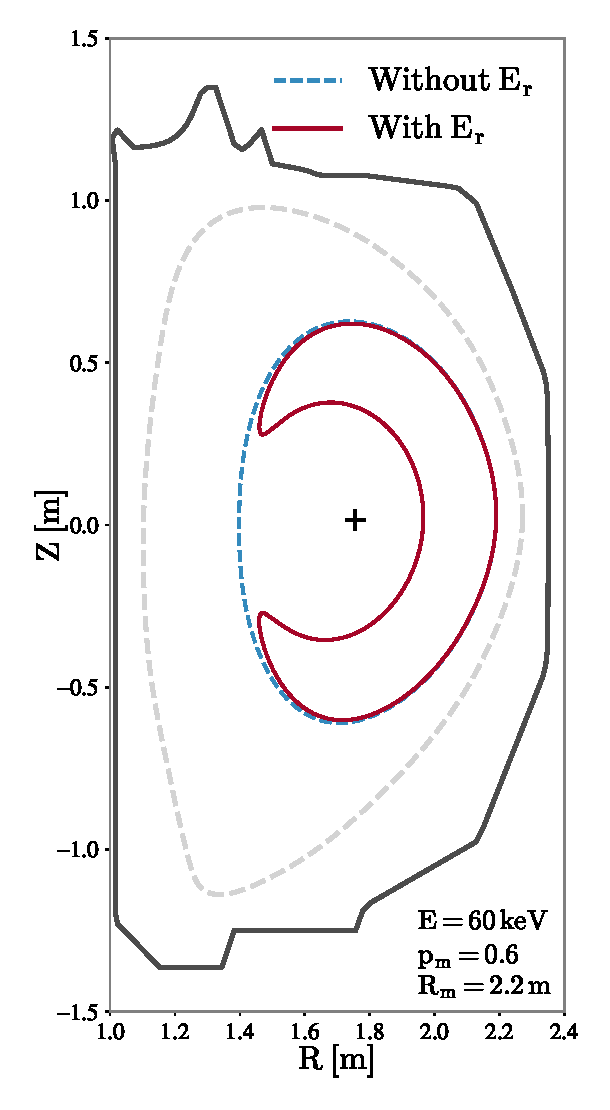
\includegraphics[width=7cm]{figures/orbit_er.eps}
    \caption{Two orbits, one including the effects of the radial electric field (red line), one without (blue dashed line). Including the radial electric field changes the orbit topology.}
    \label{fig:orbit_er}
\end{figure}
As shown in Figure \ref{fig:orbit_er}, including the effects of the radial electric field can substantially change the trajectory of the orbit and, consequentially, the orbit's weight function. For this reason, the $E \times B$ drift must be included.

The orbit coordinates, describe in the previous section, provide three out of the four initial conditions needed to solve Equation \ref{eq:gc_ode}: the kinetic energy, pitch, and $R$. The fourth initial condition is the initial $Z$ position of the fast-ion. The initial Z position is found by finding the point of minimum poloidal flux at a fixed value of major radius, $R_m$. Since fast-ions are mostly tied to a flux surface at the outermost legs of their orbits, the point of minimum flux is also a point on the orbit.

Once all the initial conditions are found, Equation \ref{eq:gc_ode} is solved for one poloidal transit time of the orbit, with particle locations and velocities dumped at equal time steps throughout the interval $[0,\tau_p)$. The particles are given equal weights and loaded into the diagnostic's forward model e.g. FIDASIM---this is equivalent to evaluating the integral in Equation \ref{eq:orbit_weight}. Orbits that are degenerate or intersect the vessel wall have null orbit weights and are excluded.

The calculation of the orbit weights can be computationally intensive. To reduce the computational time, an orbit with small time steps can be down-sampled to an orbit with larger time steps. This reduces the number of particles used in the calculation. Using a down-sampling method, instead of using a larger time step when the orbit is first calculated, perseveres the accuracy of the orbit trajectory. Typically, the down-sampling time step is chosen such that the mean poloidal distance between particles is $\sim1$ cm. An example of a down-sampled orbit is shown in Figure \ref{fig:down_sample}.
\begin{figure}[h!]
    \centering
    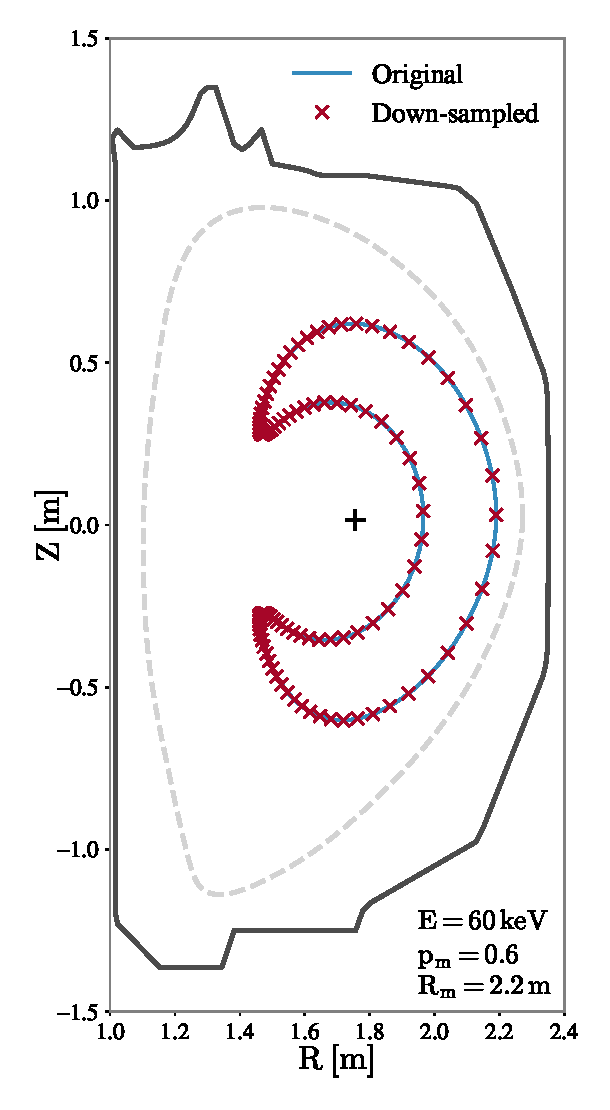
\includegraphics[width=7cm]{figures/down_sampled_orbit.eps}
    \caption{Example of a down-sampled orbit. The blue line is the original orbit and the red x's are the points used to calculate the orbit's weight function. For illustrative purposes, the mean poloidal length between points is set to 4 cm. Typically, a mean poloidal length of 1 cm is used.}
    \label{fig:down_sample}
\end{figure}

\subsection{Orbit Weight Functions for Various Fast-ion Diagnostics}
In this section, after briefly describing the plasma conditions and diagnostics,
orbit weight functions are calculated for three DIII-D fast-ion diagnostics: 
the neutron scintillator, the solid state neutral particle analyzer (ssNPA), and the fast-ion D-$\alpha$ (FIDA) spectrometer.
The orbit weight functions are calculated on a $100 \times 100 \times 100$ element 
$(E,p_m,R_m)$ grid.

\subsubsection{Apparatus} \label{sec:apparatus}
The selected plasma is 
DIII-D shot \#159243 at 790 ms. This discharge, which is discussed in detail in
 Ref. \cite{heidbrink2017}, is a reversed-shear plasma with toroidal field of 2.0 T and
plasma current of +0.8 MA (counter clockwise). The fast-ion population is created by
deuterium neutral beams of energy 70-81 keV that are injected in
both the co-current and counter-current directions. Although, the discharge has extensive Alfv\'en
eigenmode activity, only the ``classical'' distribution function calculated by NUBEAM
\cite{NUBEAM} in the absence of wave-induced transport is considered here.
Projections of the orbit-space fast-ion distribution function for the shot are shown in 
Figure \ref{fig:distribution}.
\begin{figure}[ht]
    \centering
    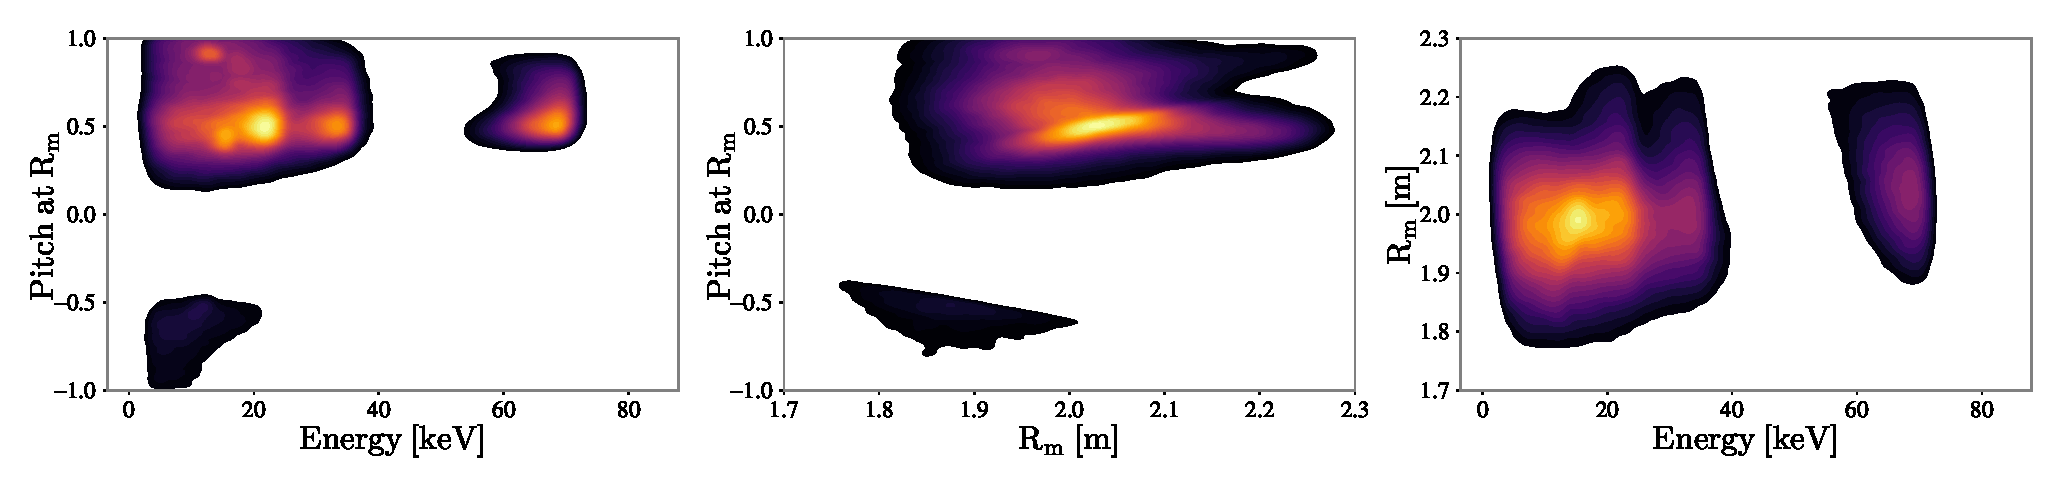
\includegraphics[width=15cm]{orbit_distribution}
    \caption{Projections of the orbit-space fast-ion distribution for shot \#159243 at 790 ms. Each projection is the full 3D distribution integrated over one of the variables e.g. $F_z(x,y) = \int F(x,y,z)\;dz$.  Each projection is normalized to unity. The color-map increases linearly from dark(black) to light(yellow).}
    \label{fig:distribution}
\end{figure}


%==============================================================================
%---------------------------------- NEUTRON -----------------------------------
%==============================================================================

%\begin{figure}[ht]
%    \centering 
%    \includegraphics[width=15cm]{neutron_cross_section}
%    \caption{Energy dependence of neutron cross section for D-D fusion reactions.}
%    \label{fig:neutron_cross_section}
%\end{figure}
\subsubsection{Neutron Scintillator Orbit Weight Function}
The neutron scintillator measures the volume-averaged neutron rate; Figure \ref{fig:neutron_orbit_weight} shows its orbit weight function.
In isolation, the neutron orbit weight function gives insight into the underlying physics of the diagnostic.
\begin{figure}[h!]
    \centering
    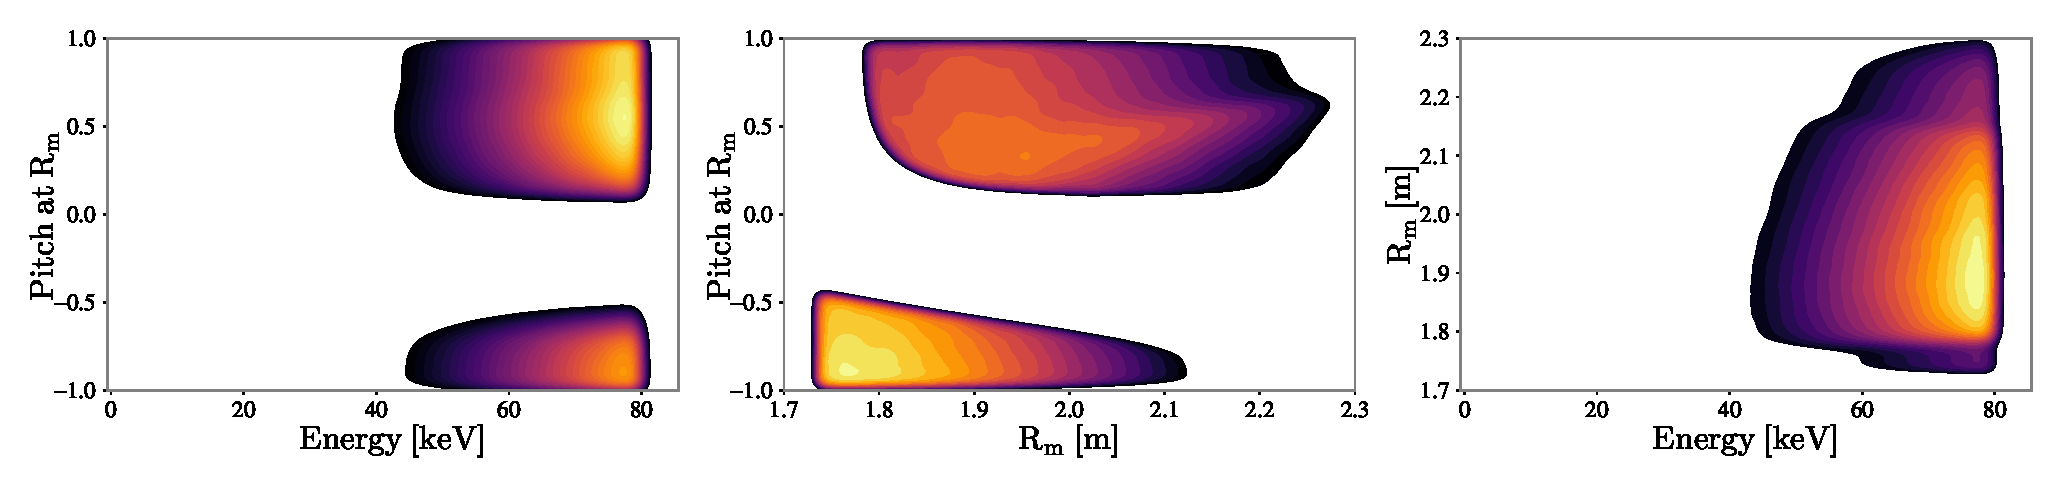
\includegraphics[width=17cm]{figures/neutron_orbit_weight.eps}
    \caption{Normalized projections of the 3D neutron orbit weight function.}
    \label{fig:neutron_orbit_weight}
\end{figure}
For example, the strong energy dependence of the orbit weight function indicates that the effect of the neutron cross section is considerable. This type of analysis can also be done using velocity-space weight functions, however, with orbit weights the sensitivity of the diagnostic to individual orbit types can also be analyzed.
\begin{table}[h!]
    \centering
    \begin{tabular}{|c|c|c|c|}
    \hline
    Orbit Type & Average Weight [$s^{-1}$] & Phase-space Fraction & Signal Produced [$s^{-1}$]\\
    \hline
    Potato      & $3.83\times10^{-5}$ & $7.75\times10^{-3}$ & $1.19\times10^{12}$  \\
    Stagnation  & $3.69\times10^{-5}$ & $9.61\times10^{-2}$ & $2.86\times10^{11}$  \\
    Trapped     & $2.09\times10^{-5}$ & $2.41\times10^{-1}$ & $5.65\times10^{12}$  \\
    Ctr-Passing & $2.82\times10^{-5}$ & $2.93\times10^{-1}$ & $3.67\times10^{11}$  \\
    Co-Passing  & $2.67\times10^{-5}$ & $3.62\times10^{-1}$ & $1.57\times10^{13}$  \\
    \hline
    Total       &                     &                     & $2.32\times10^{13}$  \\
    \hline
    \end{tabular}
    \caption{Dependence of neutron signal on orbit topology for DIII-D discharge \#159243 at 790 ms. Column~1: Type \cite{WHITE} of orbit. Column~2: Average neutron signal produced by a fast ion of the given type. Column~3: Fraction of the fast-ion phase space occupied by the orbit type. Column~4: Total neutron signal produced by each orbit type. The table indicates that the neutron diagnostic is most sensitive to potato orbits. Additionally, it shows that counter-passing orbits produce more signal on average than co-passing orbits due to counter-passing orbits traveling against the bulk plasma rotation, causing a higher relative energy. See the caption of Figure \ref{fig:orbit_topology} for explaination of the different orbit types.}
    \label{tab:neutron_orbit_weight}    
\end{table}
\begin{figure}[h!]
    \centering
    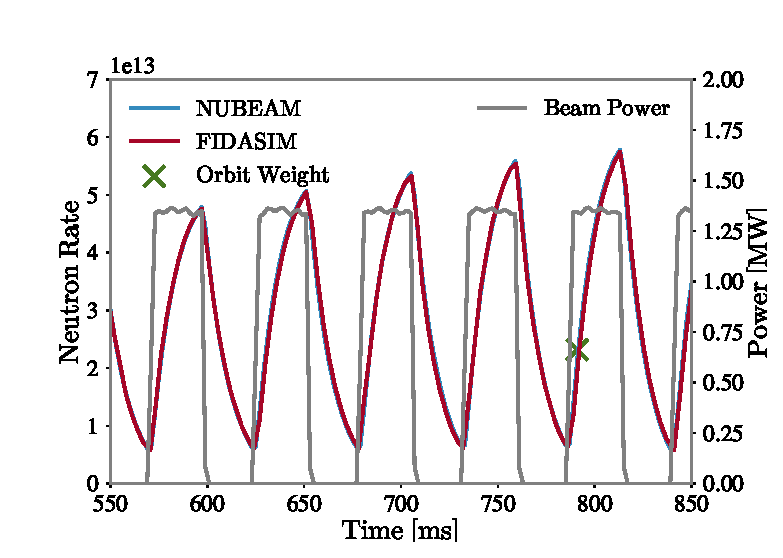
\includegraphics[width=10cm]{figures/neutron_rate.eps}
    \caption{Beam-plasma neutron rate and injected beam power over time for shot \#159243 calculated by the NUBEAM and FIDASIM codes and the rate at 790 ms calculated using the neutron orbit weight function and Equation \ref{eq:orbit_tomography}.}
    \label{fig:neutron_rate}
\end{figure}
Table \ref{tab:neutron_orbit_weight} shows the signal produced by each orbit type, indicating that co-passing orbits produce the most signal. Somewhat surprisingly, the neutron diagnostic is quite sensitive to potato orbits despite the small volume of phase space that they occupy. This is caused by the tendency of potato orbits to spend a large fraction of their orbit in the high density core region. 
The total beam-plasma neutrons produced, as calculated by Equation \ref{eq:orbit_tomography}, is in agreement with the predictions of TRANSP/NUBEAM and FIDASIM (Fig. \ref{fig:neutron_rate}).
\begin{figure}[h!]
    \centering
    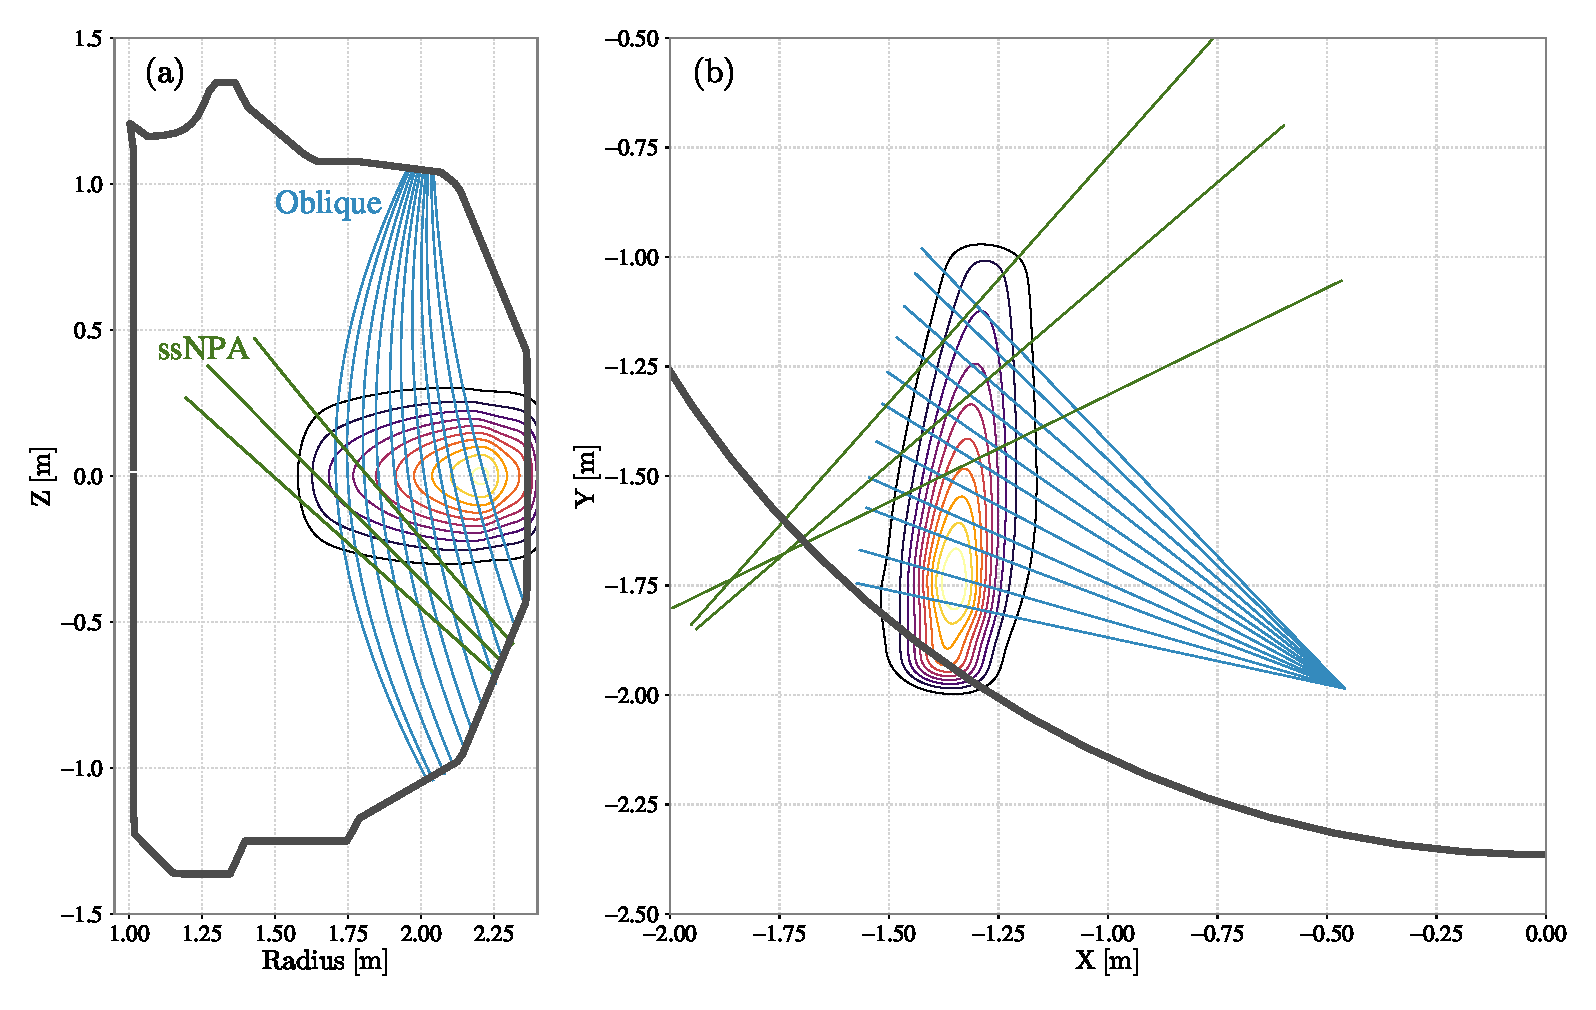
\includegraphics[width=15cm]{figures/geometry.eps}
    \caption{Poloidal (a) and plan (b) view of the 210RT neutral beam density (contours) and fast-ion diagnostics (colored lines). The Oblique FIDA system\cite{muscatello2010}, shown in blue, consists of of a maximum of 11 viewing chords looking down at the 210RT beam at an oblique angle of 
$\sim45^{\circ}$ with respect to the midplane. The solid state NPA system (ssNPA)\cite{ssNPA2012}, shown in green, consists of three channels viewing the core region of the plasma from below the midplane.}
    \label{fig:geometry}
\end{figure}

\subsubsection{NPA Orbit Weight Function}
The solid state NPA (ssNPA) diagnostic measures fast neutrals, born of charge exchange, that escape the plasma. DIII-D utilizes three separate channels, each viewing the 210RT neutral beam at a different radial location (Fig. \ref{fig:geometry}). In its present configuration, the detectors are operated in current mode \cite{ssNPA2012}.
Figure \ref{fig:npa_orbit_weight} shows the orbit weight function for the central channel. Upon inspection, it shows that the ssNPA diagnostic is localized in space ($R_m$) and in pitch ($p_m$) but, because the detector is operated in current mode, it is also sensitive to a large swath of energies. The localization in space and pitch is caused by the narrow collimation of the diagnostic. In a three dimensional view, the orbit weight function is characterized as a line through the orbit-space. As an aside, the previously discussed imaging NPA\cite{du2018inpa}, which is similarly localized in pitch but has an extended radial view, has an orbit weight function that takes the form of a 2d surface within the 3D orbit-space.
\begin{figure}[h!]
    \centering
    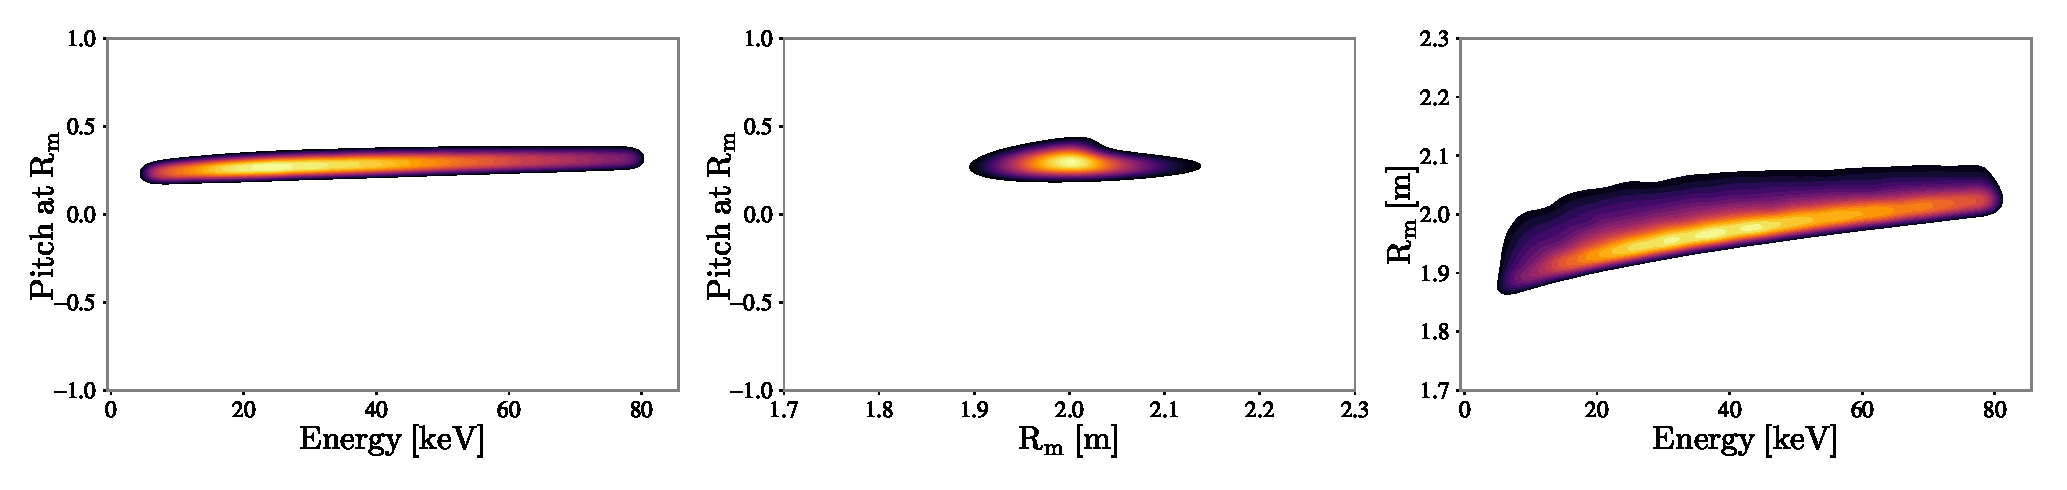
\includegraphics[width=15cm]{figures/npa_orbit_weight_2.eps}
    \caption{Normalized projections of the ssNPA(Fig. \ref{fig:geometry}) orbit weight function at R=1.64 m for shot \#159243 @ 790 ms}
    \label{fig:npa_orbit_weight}
\end{figure}

Providing further evidence that the orbit weight functions faithfully encode the ssNPA's full forward model, Figure \ref{fig:npa_ow_flux} shows that the energy resolved NPA flux calculated using the NPA orbit weights agrees with FIDASIM. 
\begin{figure}[h!]
    \centering
    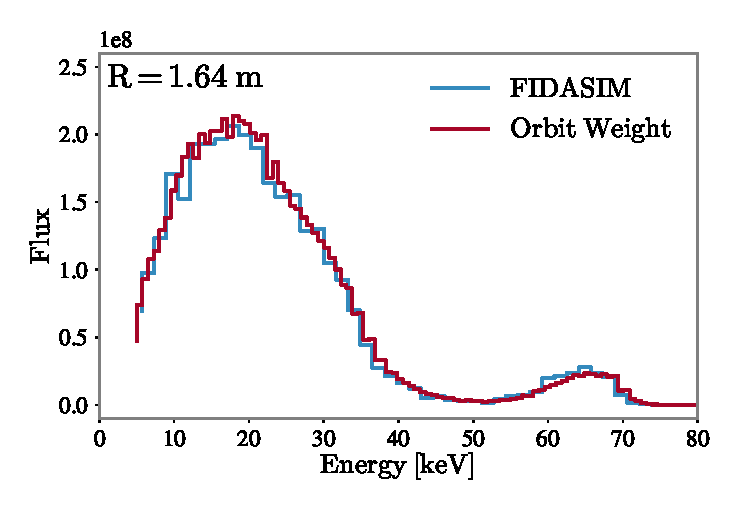
\includegraphics[width=10cm]{figures/npa_flux.eps}
    \caption{Comparison of the energy resolved ssNPA flux for shot \#159243 @ 790 ms calculated by FIDASIM and by the NPA orbit weight functions and Equation \ref{eq:orbit_tomography}.}
    \label{fig:npa_ow_flux}
\end{figure}

\subsubsection{Fast-ion D-$\alpha$ Spectroscopy (FIDA) Orbit Weight Function}
The main FIDA system used at DIII-D is the Oblique FIDA system (Fig. \ref{fig:geometry}), which consists of an array of radial views of the 210RT neutral beam.
The FIDA orbit weight functions depend on wavelength.
For instance, if we consider the orbit weight function for a red shifted wavelength (Fig. \ref{fig:fida_red}) we can see that the chord (oblique@1.9m) sees signal from counter-passing particles localized at $R_m$=1.91 m and also trapped particles from as far out as $R_m$=2.18 m. 
\begin{figure}[h!]
    \centering
    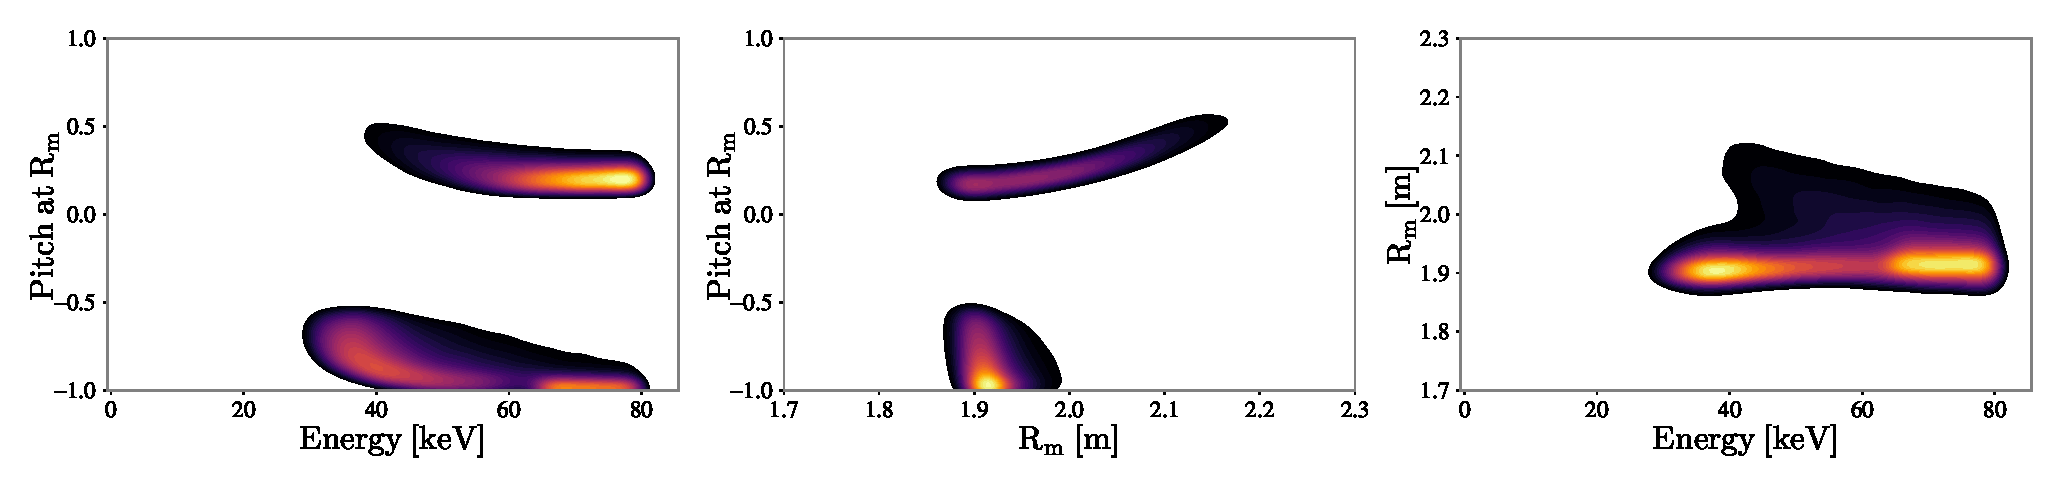
\includegraphics[width=15cm]{figures/fida_orbit_weight_red_14.eps}
    \caption{Projections of the red shifted ($\lambda = 660 \pm 0.2$ nm) FIDA orbit weight function for an oblique viewing chord with midplane intersection at R=1.9 m.}
    \label{fig:fida_red}
\end{figure}

We can also view the orbit weight function for a blue shifted wavelength for the same radial position (Fig. \ref{fig:fida_blue}). 
\begin{figure}[h!]
    \centering
    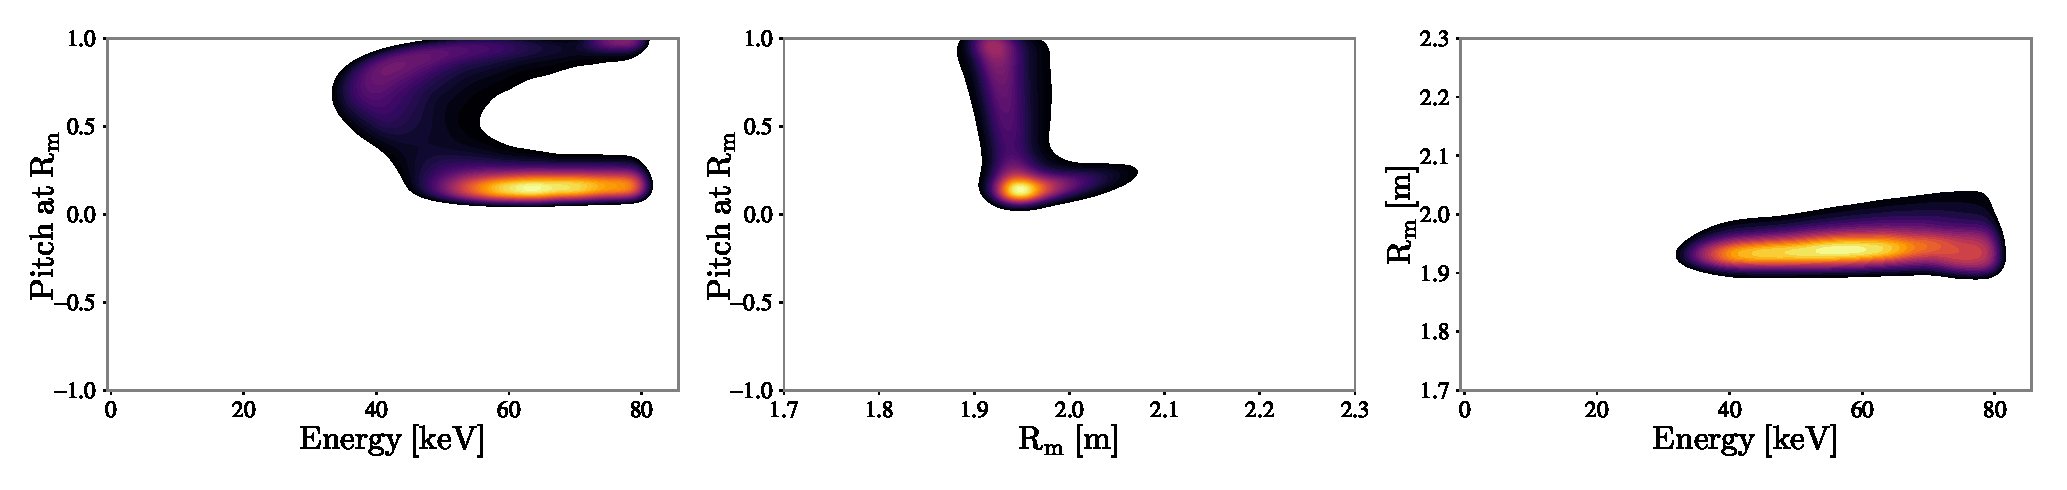
\includegraphics[width=15cm]{figures/fida_orbit_weight_blue_14.eps}
    \caption{Projections of the blue shifted ($\lambda = 652 \pm 0.2$ nm) FIDA orbit weight function for an oblique viewing chord with midplane intersection at R=1.9 m.}
    \label{fig:fida_blue}
\end{figure}
Unlike the red shifted orbit weight function the blue shifted weight function is not sensitive to counter-passing particles, only showing sensitivity to orbits that are co-passing in the viewing region.

Like the other diagnostics, the spectra calculated using orbit weight functions closely matches the spectra produced by FIDASIM (Fig. \ref{fig:fida_orbit_spectra}). Also compared in the figure is the spectra calculated using velocity-space weight functions, which performs poorly in this case.
\begin{figure}[h!]
    \centering
    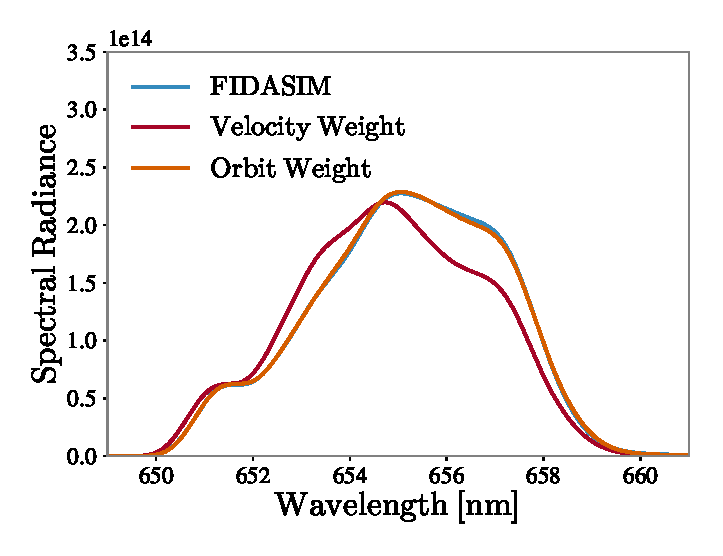
\includegraphics[width=10cm]{figures/fida_orbit_spectra.eps}
    \caption{FIDA Spectra for shot \#159243 @ 790 ms calculated by FIDASIM and by the FIDA orbit weight functions and Equation \ref{eq:orbit_tomography} for an oblique (Fig. \ref{fig:geometry}) viewing chord at $R = 2.1$ m.}
    \label{fig:fida_orbit_spectra}
\end{figure}



